\documentclass{beamer}

\usetheme{Warsaw}
\usepackage{graphicx}
\usepackage{ulem}
\usepackage{tikz}
\usepackage{subcaption}
% include.tex
\newcommand{\Bernoulli}[1]{\text{Bernoulli} \left( #1 \right)}
\newcommand{\mydigamma}[1]{\psi \left( #1 \right)}
%\newcommand{\diag}[1]{\text{diag}\left( #1 \right)}
\newcommand{\tr}[1]{\text{tr}\left( #1 \right)}
\newcommand{\Poisson}[1]{\text{Poisson} \left( #1 \right)}
\def \half {\frac{1}{2}}
\def \R {\mathbb{R}}
\def \vbeta {\vec{\beta}}
\def \vy {\vec{y}}
\def \vmu {\vec{\mu}}
\def \vmuqbeta {\vmu_{q(\vbeta)}}
\def \vmubeta {\vmu_{\vbeta}}
\def \Sigmaqbeta {\Sigma_{q(\vbeta)}}
\def \Sigmabeta {\Sigma_{\vbeta}}
\def \va {\vec{a}}
\def \vtheta {\vec{\theta}}
\def \mX {\vec{X}}

\def\ds{{\displaystyle}}

\def\diag{{\mbox{diag}}}


\usepackage{latexsym,amssymb,amsmath,amsfonts}
%\usepackage{tabularx}
\usepackage{theorem}
\usepackage{verbatim,array,multicol,palatino}
\usepackage{graphicx}
\usepackage{graphics}
\usepackage{fancyhdr}
\usepackage{algorithm,algorithmic}
\usepackage{url}
%\usepackage[all]{xy}



\def\approxdist{\stackrel{{\tiny \mbox{approx.}}}{\sim}}
\def\smhalf{\textstyle{\frac{1}{2}}}
\def\vxnew{\vx_{\mbox{{\tiny new}}}}
\def\bib{\vskip12pt\par\noindent\hangindent=1 true cm\hangafter=1}
\def\jump{\vskip3mm\noindent}
\def\etal{{\em et al.}}
\def\etahat{{\widehat\eta}}
\def\thick#1{\hbox{\rlap{$#1$}\kern0.25pt\rlap{$#1$}\kern0.25pt$#1$}}
\def\smbbeta{{\thick{\scriptstyle{\beta}}}}
\def\smbtheta{{\thick{\scriptstyle{\theta}}}}
\def\smbu{{\thick{\scriptstyle{\rm u}}}}
\def\smbzero{{\thick{\scriptstyle{0}}}}
\def\boxit#1{\begin{center}\fbox{#1}\end{center}}
\def\lboxit#1{\vbox{\hrule\hbox{\vrule\kern6pt
      \vbox{\kern6pt#1\kern6pt}\kern6pt\vrule}\hrule}}
\def\thickboxit#1{\vbox{{\hrule height 1mm}\hbox{{\vrule width 1mm}\kern6pt
          \vbox{\kern6pt#1\kern6pt}\kern6pt{\vrule width 1mm}}
               {\hrule height 1mm}}}


%\sloppy
%\usepackage{geometry}
%\geometry{verbose,a4paper,tmargin=20mm,bmargin=20mm,lmargin=40mm,rmargin=20mm}


%%%%%%%%%%%%%%%%%%%%%%%%%%%%%%%%%%%%%%%%%%%%%%%%%%%%%%%%%%%%%%%%%%%%%%%%%%%%%%%%
%
% Some convenience definitions
%
% \bf      -> vector
% \sf      -> matrix
% \mathcal -> sets or statistical
% \mathbb  -> fields or statistical
%
%%%%%%%%%%%%%%%%%%%%%%%%%%%%%%%%%%%%%%%%%%%%%%%%%%%%%%%%%%%%%%%%%%%%%%%%%%%%%%%%

% Sets or statistical values
\def\sI{{\mathcal I}}                            % Current Index set
\def\sJ{{\mathcal J}}                            % Select Index set
\def\sL{{\mathcal L}}                            % Likelihood
\def\sl{{\ell}}                                  % Log-likelihood
\def\sN{{\mathcal N}}                            
\def\sS{{\mathcal S}}                            
\def\sP{{\mathcal P}}                            
\def\sQ{{\mathcal Q}}                            
\def\sB{{\mathcal B}}                            
\def\sD{{\mathcal D}}                            
\def\sT{{\mathcal T}}
\def\sE{{\mathcal E}}                            
\def\sF{{\mathcal F}}                            
\def\sC{{\mathcal C}}                            
\def\sO{{\mathcal O}}                            
\def\sH{{\mathcal H}} 
\def\sR{{\mathcal R}}                            
\def\sJ{{\mathcal J}}                            
\def\sCP{{\mathcal CP}}                            
\def\sX{{\mathcal X}}                            
\def\sA{{\mathcal A}} 
\def\sZ{{\mathcal Z}}                            
\def\sM{{\mathcal M}}                            
\def\sK{{\mathcal K}}     
\def\sG{{\mathcal G}}                         
\def\sY{{\mathcal Y}}                         
\def\sU{{\mathcal U}}  


\def\sIG{{\mathcal IG}}                            


\def\cD{{\sf D}}
\def\cH{{\sf H}}
\def\cI{{\sf I}}

% Vectors
\def\vectorfontone{\bf}
\def\vectorfonttwo{\boldsymbol}
\def\va{{\vectorfontone a}}                      %
\def\vb{{\vectorfontone b}}                      %
\def\vc{{\vectorfontone c}}                      %
\def\vd{{\vectorfontone d}}                      %
\def\ve{{\vectorfontone e}}                      %
\def\vf{{\vectorfontone f}}                      %
\def\vg{{\vectorfontone g}}                      %
\def\vh{{\vectorfontone h}}                      %
\def\vi{{\vectorfontone i}}                      %
\def\vj{{\vectorfontone j}}                      %
\def\vk{{\vectorfontone k}}                      %
\def\vl{{\vectorfontone l}}                      %
\def\vm{{\vectorfontone m}}                      % number of basis functions
\def\vn{{\vectorfontone n}}                      % number of training samples
\def\vo{{\vectorfontone o}}                      %
\def\vp{{\vectorfontone p}}                      % number of unpenalized coefficients
\def\vq{{\vectorfontone q}}                      % number of penalized coefficients
\def\vr{{\vectorfontone r}}                      %
\def\vs{{\vectorfontone s}}                      %
\def\vt{{\vectorfontone t}}                      %
\def\vu{{\vectorfontone u}}                      % Penalized coefficients
\def\vv{{\vectorfontone v}}                      %
\def\vw{{\vectorfontone w}}                      %
\def\vx{{\vectorfontone x}}                      % Covariates/Predictors
\def\vy{{\vectorfontone y}}                      % Targets/Labels
\def\vz{{\vectorfontone z}}                      %

\def\vone{{\vectorfontone 1}}
\def\vzero{{\vectorfontone 0}}

\def\valpha{{\vectorfonttwo \alpha}}             %
\def\vbeta{{\vectorfonttwo \beta}}               % Unpenalized coefficients
\def\vgamma{{\vectorfonttwo \gamma}}             %
\def\vdelta{{\vectorfonttwo \delta}}             %
\def\vepsilon{{\vectorfonttwo \epsilon}}         %
\def\vvarepsilon{{\vectorfonttwo \varepsilon}}   % Vector of errors
\def\vzeta{{\vectorfonttwo \zeta}}               %
\def\veta{{\vectorfonttwo \eta}}                 % Vector of natural parameters
\def\vtheta{{\vectorfonttwo \theta}}             % Vector of combined coefficients
\def\vvartheta{{\vectorfonttwo \vartheta}}       %
\def\viota{{\vectorfonttwo \iota}}               %
\def\vkappa{{\vectorfonttwo \kappa}}             %
\def\vlambda{{\vectorfonttwo \lambda}}           % Vector of smoothing parameters
\def\vmu{{\vectorfonttwo \mu}}                   % Vector of means
\def\vnu{{\vectorfonttwo \nu}}                   %
\def\vxi{{\vectorfonttwo \xi}}                   %
\def\vpi{{\vectorfonttwo \pi}}                   %
\def\vvarpi{{\vectorfonttwo \varpi}}             %
\def\vrho{{\vectorfonttwo \rho}}                 %
\def\vvarrho{{\vectorfonttwo \varrho}}           %
\def\vsigma{{\vectorfonttwo \sigma}}             %
\def\vvarsigma{{\vectorfonttwo \varsigma}}       %
\def\vtau{{\vectorfonttwo \tau}}                 %
\def\vupsilon{{\vectorfonttwo \upsilon}}         %
\def\vphi{{\vectorfonttwo \phi}}                 %
\def\vvarphi{{\vectorfonttwo \varphi}}           %
\def\vchi{{\vectorfonttwo \chi}}                 %
\def\vpsi{{\vectorfonttwo \psi}}                 %
\def\vomega{{\vectorfonttwo \omega}}             %


% Matrices
%\def\matrixfontone{\sf}
%\def\matrixfonttwo{\sf}
\def\matrixfontone{\bf}
\def\matrixfonttwo{\boldsymbol}
\def\mA{{\matrixfontone A}}                      %
\def\mB{{\matrixfontone B}}                      %
\def\mC{{\matrixfontone C}}                      % Combined Design Matrix
\def\mD{{\matrixfontone D}}                      % Penalty Matrix for \vu_J
\def\mE{{\matrixfontone E}}                      %
\def\mF{{\matrixfontone F}}                      %
\def\mG{{\matrixfontone G}}                      % Penalty Matrix for \vu
\def\mH{{\matrixfontone H}}                      %
\def\mI{{\matrixfontone I}}                      % Identity Matrix
\def\mJ{{\matrixfontone J}}                      %
\def\mK{{\matrixfontone K}}                      %
\def\mL{{\matrixfontone L}}                      % Lower bound
\def\mM{{\matrixfontone M}}                      %
\def\mN{{\matrixfontone N}}                      %
\def\mO{{\matrixfontone O}}                      %
\def\mP{{\matrixfontone P}}                      %
\def\mQ{{\matrixfontone Q}}                      %
\def\mR{{\matrixfontone R}}                      %
\def\mS{{\matrixfontone S}}                      %
\def\mT{{\matrixfontone T}}                      %
\def\mU{{\matrixfontone U}}                      % Upper bound
\def\mV{{\matrixfontone V}}                      %
\def\mW{{\matrixfontone W}}                      % Variance Matrix i.e. diag(b'')
\def\mX{{\matrixfontone X}}                      % Unpenalized Design Matrix/Nullspace Matrix
\def\mY{{\matrixfontone Y}}                      %
\def\mZ{{\matrixfontone Z}}                      % Penalized Design Matrix/Kernel Space Matrix

\def\mGamma{{\matrixfonttwo \Gamma}}             %
\def\mDelta{{\matrixfonttwo \Delta}}             %
\def\mTheta{{\matrixfonttwo \Theta}}             %
\def\mLambda{{\matrixfonttwo \Lambda}}           % Penalty Matrix for \vnu
\def\mXi{{\matrixfonttwo \Xi}}                   %
\def\mPi{{\matrixfonttwo \Pi}}                   %
\def\mSigma{{\matrixfonttwo \Sigma}}             %
\def\mUpsilon{{\matrixfonttwo \Upsilon}}         %
\def\mPhi{{\matrixfonttwo \Phi}}                 %
\def\mOmega{{\matrixfonttwo \Omega}}             %
\def\mPsi{{\matrixfonttwo \Psi}}                 %

\def\mone{{\matrixfontone 1}}
\def\mzero{{\matrixfontone 0}}

% Fields or Statistical
\def\bE{{\mathbb E}}                             % Expectation
\def\bP{{\mathbb P}}                             % Probability
\def\bR{{\mathbb R}}                             % Reals
\def\bI{{\mathbb I}}                             % Reals
\def\bV{{\mathbb V}}                             % Reals

\def\vX{{\vectorfontone X}}                      % Targets/Labels
\def\vY{{\vectorfontone Y}}                      % Targets/Labels
\def\vZ{{\vectorfontone Z}}                      %

% Other
\def\etal{{\em et al.}}
\def\ds{\displaystyle}
\def\d{\partial}
\def\diag{\text{diag}}
%\def\span{\text{span}}
\def\blockdiag{\text{blockdiag}}
\def\tr{\text{tr}}
\def\RSS{\text{RSS}}
\def\df{\text{df}}
\def\GCV{\text{GCV}}
\def\AIC{\text{AIC}}
\def\MLC{\text{MLC}}
\def\mAIC{\text{mAIC}}
\def\cAIC{\text{cAIC}}
\def\rank{\text{rank}}
\def\MASE{\text{MASE}}
\def\SMSE{\text{SASE}}
\def\sign{\text{sign}}
\def\card{\text{card}}
\def\notexp{\text{notexp}}
\def\ASE{\text{ASE}}
\def\ML{\text{ML}}
\def\nullity{\text{nullity}}

\def\logexpit{\text{logexpit}}
\def\logit{\mbox{logit}}
\def\dg{\mbox{dg}}

\def\Bern{\mbox{Bernoulli}}
\def\sBernoulli{\mbox{Bernoulli}}
\def\sGamma{\mbox{Gamma}}
\def\sInvN{\mbox{Inv}\sN}
\def\sNegBin{\sN\sB}

\def\dGamma{\mbox{Gamma}}
\def\dInvGam{\mbox{Inv}\Gamma}

\def\Cov{\mbox{Cov}}
\def\Mgf{\mbox{Mgf}}

\def\mis{{mis}} 
\def\obs{{obs}}

\def\argmax{\operatornamewithlimits{\text{argmax}}}
\def\argmin{\operatornamewithlimits{\text{argmin}}}
\def\argsup{\operatornamewithlimits{\text{argsup}}}
\def\arginf{\operatornamewithlimits{\text{arginf}}}


\def\minimize{\operatornamewithlimits{\text{minimize}}}
\def\maximize{\operatornamewithlimits{\text{maximize}}}
\def\suchthat{\text{such that}}


\def\relstack#1#2{\mathop{#1}\limits_{#2}}
\def\sfrac#1#2{{\textstyle{\frac{#1}{#2}}}}


\def\comment#1{
\vspace{0.5cm}
\noindent \begin{tabular}{|p{14cm}|}  
\hline #1 \\ 
\hline 
\end{tabular}
\vspace{0.5cm}
}


\def\mytext#1{\begin{tabular}{p{13cm}}#1\end{tabular}}
\def\mytextB#1{\begin{tabular}{p{7.5cm}}#1\end{tabular}}
\def\mytextC#1{\begin{tabular}{p{12cm}}#1\end{tabular}}

\def\jump{\vskip3mm\noindent}

\def\KL{\text{KL}}
\def\N{\text{N}}
\def\Var{\text{Var}}

\def \E {\mathbb{E}}
\def \BigO {\text{O}}
\def \IG {\text{IG}}
\def \Beta {\text{Beta}}



\usefonttheme{serif}

\title{Gaussian Variational Bayes approximations to zero--inflated mixed models}
\author{Mark Greenaway}

\mode<presentation>
{ \usetheme{boxes} }

\begin{document}
% 1. Front slide
\begin{frame}
	\titlepage
	% Details about myself here?
\end{frame}

% 2. Intro
\begin{frame}
	\frametitle{Introduction}
	Zero inflated data arises in many areas of application, such as physical
	activity data, number of hospital visits per year per person and
	number of insurance claims per year per person.
			
	\bigskip 
	We will work with zero-inflated count data. I encountered this sort of data 
	while analysing physical activity data arising from the Get Healthy project.
\end{frame}

% 4. \rho = 9/10, \lambda = 5
% Example data 0 0 0 5 10
\begin{frame}[fragile]
	\frametitle{Example data}
	Consider the following counts:
	\begin{verbatim}
0 7 3 4 5 3 2 6 5 0 0 1
0 0 5 0 2 3 6 4 0 5 4 0
7 0 0 0 7 0 6 6 0 3 0 5
0 4 0 0 0 2 3 0 3 4 5 0
8 0
	\end{verbatim}
	%Take, for example, $\rho = \frac{1}{2}, \lambda = 5$.
			
	\noindent Note that $n=50$, 
	$n\times P(Z = 0) \approx 3.8$ for $Z\sim\mbox{Poisson}(\overline{X})$
	where $\overline{X}$ is the mean of the count data and we have observed 21 zeros. This suggests
	a Poisson model is not suitable.
			
	% Histogram
	\begin{figure}
		% 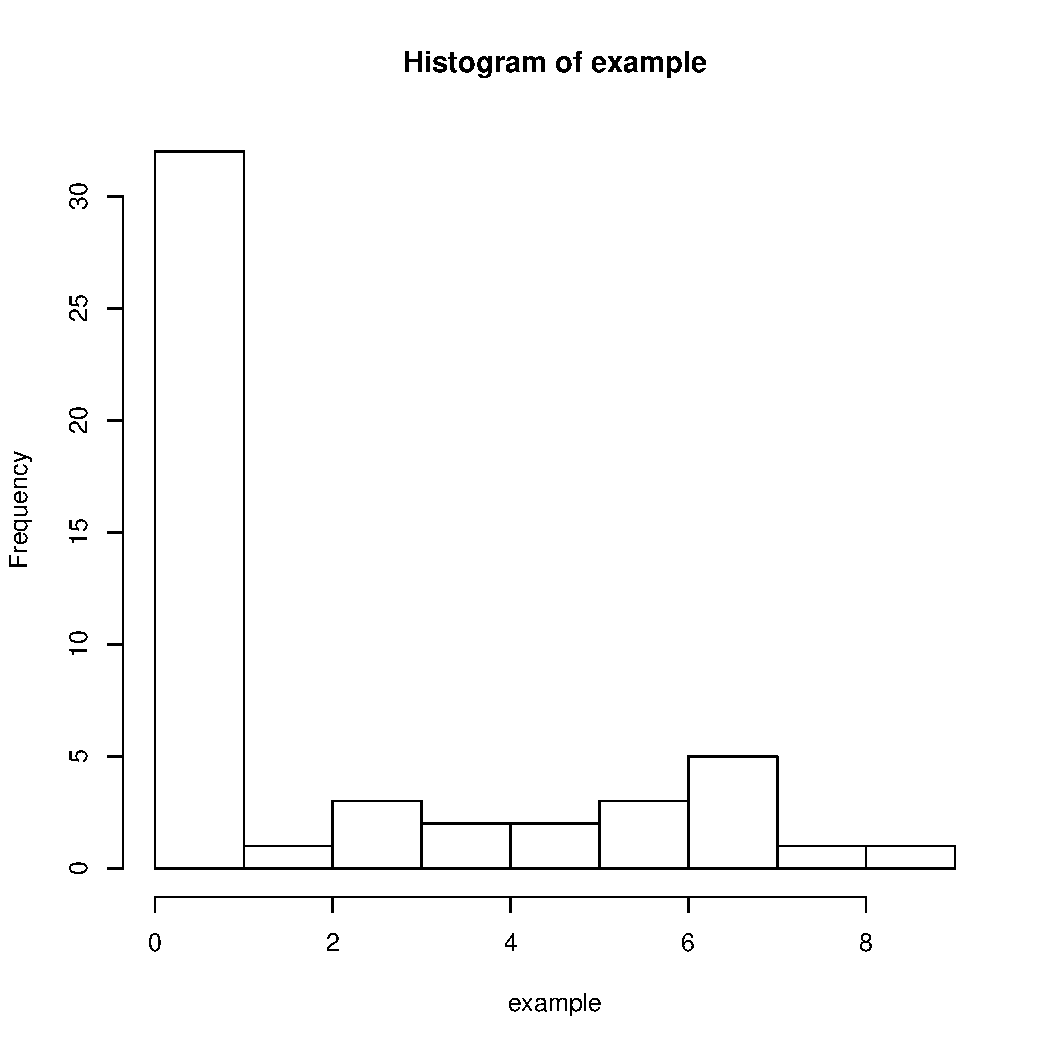
\includegraphics[width=50mm, height=50mm]{code/results/univariate_data_histogram.pdf}
		% pdf("~/Dropbox/phd/poisson_does_not_fit.pdf")
		% hist(x, , prob=TRUE)
		% points(0:8 + .5, dpois(0:8, lambda_hat), col = "red")
		% dev.off()
		\includegraphics[width=50mm, height=50mm]{poisson_does_not_fit.pdf}
	\end{figure}% Density
\end{frame}


\begin{frame}
	\frametitle{Multivariate model formulation}
	We use a zero-inflated Poisson random effects model.
			
	\medskip
			
	Suppose that we observe a vector of responses $\vy$ of length n, and matrices
	of covariates $\mX$ and $\mZ$ of dimensions $n \times p$ and $n \times m$,
	respectively.
			
	\begin{align*}
		p(\vy|\vbeta, \vu, \vr)       & = \exp{\left[\vy^\top \mR(\mX \vbeta + \mZ \vu) - \vr^\top e^{\mX \vbeta + \mZ \vu} - \vone^\top \log{(\vy !)}\right]}, \\
		\vr_i|\rho                    & \stackrel{\mbox{\tiny iid}}{\sim} \text{Bernoulli}(\rho), \ \{i \colon \vy_i=0\},                                       \\
		\text{and }\vu|\sigma_{\vu}^2 & \sim \N({\bf 0}, \sigma_{\vu}^2 \mI)                                                                                    \\
	\end{align*}
	\noindent where $\mR =\mbox{diag}(\vr)$.
	We use the priors:
	\begin{align*}
		\vbeta          & \sim \text{N}({\bf 0}, \sigma_\vbeta^2\mI),                  \\
		\sigma_\vu^2    & \sim \text{IG}(\alpha_{\sigma_\vu^2}, \beta_{\sigma_\vu^2}), \\
		\text{and }\rho & \sim \text{Beta}(a_\rho, b_\rho)                             \\
	\end{align*}
\end{frame}


% 3. Univariate model
\begin{frame}
	\frametitle{Latent variable formulation of zero--inflated model}
			
	\begin{columns}
		\begin{column}{0.7 \textwidth}
							
			Suppose that we observe
			$$
			Y_i = R_i X_i, \quad 1\le i\le n,
			$$
							
			\noindent where for $1\le i\le n$,
			\begin{align*} 
				R_i | \rho & \sim \text{Bernoulli}(\rho) \text{ and} \\
				X_i | \lambda & \sim \text{Poisson}(\lambda)            
			\end{align*}
							
			\noindent for parameters $\rho$ and $\lambda$,
			We use the priors:
			\begin{align*} 
				\rho    & \sim \text{Beta}(a_\rho, b_\rho)         \\
				\lambda & \sim \text{Gamma}(a_\lambda, b_\lambda). 
			\end{align*}
		\end{column}
				
		\begin{column}{0.2 \textwidth}
			\begin{figure}
				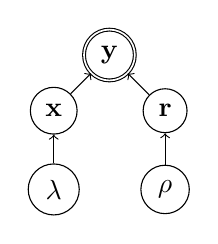
\begin{tikzpicture}
					\node[draw, circle, double] (y) {$\vy$};
					\node[draw, circle, below left of=y] (x) {$\vx$};
					\node[draw, circle, below of=x] (lambda) {$\lambda$};
					\node[draw, circle, below right of=y] (r) {$\vr$};
					\node[draw, circle, below of=r] (rho) {$\rho$};
					\draw[<-] (y) -- (x);
					\draw[<-] (x) -- (lambda);
					\draw[<-] (y) -- (r);
					\draw[<-] (r) -- (rho);
				\end{tikzpicture}
				\caption{Latent variable formulation of zero--inflated model}
			\end{figure}
		\end{column}
	\end{columns}
\end{frame}

\begin{frame}
	\frametitle{Extending to a multivariate mixed effects model}
	\begin{figure}[h]
		\centering
		\begin{subfigure}[b]{0.4 \textwidth}
			\centering
			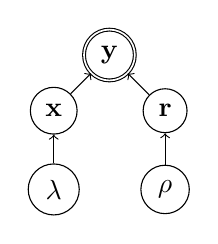
\begin{tikzpicture}
				\node[draw, circle, double] (y) {$\vy$};
				\node[draw, circle, below left of=y] (x) {$\vx$};
				\node[draw, circle, below of=x] (lambda) {$\lambda$};
				\node[draw, circle, below right of=y] (r) {$\vr$};
				\node[draw, circle, below of=r] (rho) {$\rho$};
				\draw[<-] (y) -- (x);
				\draw[<-] (x) -- (lambda);
				\draw[<-] (y) -- (r);
				\draw[<-] (r) -- (rho);
			\end{tikzpicture}
			\caption{Latent variable formulation of zero--inflated model}
		\end{subfigure}
		\begin{subfigure}[b]{0.4 \textwidth}
			\centering
			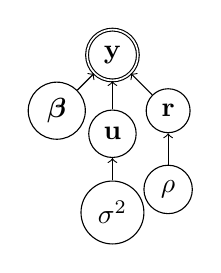
\begin{tikzpicture}
				\node[draw, circle, double] (y) {$\vy$};
				\node[draw, circle, below left of=y] (beta) {$\vbeta$};
				\node[draw, circle, below of=y] (u) {$\vu$};
				\node[draw, circle, below right of=y] (r) {$\vr$};
				\node[draw, circle, below of=u] (sigma2) {$\sigma^2$};
				\node[draw, circle, below of=r] (rho) {$\rho$};
				\draw[<-] (y) -- (beta);
				\draw[<-] (y) -- (u);
				\draw[<-] (y) -- (r);
				\draw[<-] (u) -- (sigma2);
				\draw[<-] (r) -- (rho);
			\end{tikzpicture}
			\caption{Mixed model extension of zero--inflated model}
		\end{subfigure}
	\end{figure}
		
\end{frame}

% 9. Extension to linear model
% 10. Overview GVA
% 11. Algorithm
% 12. Results?
% 13. What next
% 14. Conclusion
% 15. References
% \begin{frame}
% 	\frametitle{Extension to multivariate/regression models}
% 	\begin{itemize}
% 		\item Univariate models are a nice proof of concept.
% 		\item Most applied statisticians want to build regression models.
% 		\item Applied statisticians love mixed models.
% 		\item There is a need for better approaches to fitting zero-inflated mixed models.
% 		\item For example, MCMC with existing software can take minutes to hours 
% 		      to converge, or not converge at all.
% 		\item Not practical for many applications.
% 	\end{itemize}
% \end{frame}



% \begin{frame}
% 	\frametitle{Linear mixed model set-up}
% 	% Let $\vone$ be a vector of $1$s, and $\vone_n$ be a vector of $1$s of
% 	% length $n$.
	
% 	% TODO: Where are the prior specifications. Is this entirely accurate? What about for the random
% 	% slopes model?
		
% 	Consider a linear random intercept model with
% 	$$
% 	\begin{array}{ll}
% 		\vy|\vbeta,\vu,\sigma_y^2 & \sim \N(\mX \vbeta + \mZ \vu, \sigma_\vy^2 \mI)  \\[2ex]
% 		\vbeta                    & \sim \N(\vzero, \sigma_\vbeta^2 \mI) \text{ and} \\[2ex]
% 		\vu|\sigma_{\vu}^2        & \sim \N(\vzero, \sigma_{\vu}^2 \mI).             
% 	\end{array}
% 	$$
% 	\noindent where
% 	$$
% 	\begin{array}{rll}
% 		            & \vy    & =                                 
% 		\begin{pmatrix}
% 		y_1 \\
% 		\vdots \\
% 		y_n
% 		\end{pmatrix}, \\[2ex]
% 		            & \mX    & = [\vone_n, \vx_1, \cdots, \vx_p] \\
% 		            & \mZ    & =                                 
% 		\begin{bmatrix}
% 		\vone_{n_1} &        &                                   \\
% 		            & \ddots &                                   \\
% 		            &        & \vone_{n_m}                       
% 		\end{bmatrix} \\
% 		\text{and}  & \mC    & = [\mX, \mZ].                     
% 	\end{array}
% 	$$
% \end{frame}




% 5. How to fit, and advantages and disadvantages of each approach
% - Maximum likelihood
% - MCMC
% - VB

\begin{frame}
	\frametitle{Comparison of fitting techniques}
	\begin{tabular}{p{2cm}p{3.5cm}p{4.5cm}}
		Technique         & Pro                                                             & Con                                          \\
		\hline
		MLE               & EM could be used to fit these models, with $R_i$ as latent data & Not flexible to complications.               \\
		                  &                                                                 &                                              \\ %Frequentist \\
		\hline
		MCMC              & Bayesian                                                        & Slow                                         \\
		                  & Very accurate                                                   &                                              \\
		\hline
		Variational Bayes & Bayesian                                                        & May lose accuracy, or underestimate variance \\
		                  & Fast                                                            &                                              \\ %Solution may be intractable \\ 
		                  & Still quite accurate                                            &                                              \\
		\hline
	\end{tabular}
			
\end{frame}

% 6. Overview of Variational Bayes
\begin{frame}
	\frametitle{An overview of Variational Bayes}
	\begin{itemize}
		\item \emph{Idea:} Approximate the full posterior $p(\theta|\vy)$ with a simpler approximation $q(\vtheta)$.
		      		      		      
		\item Fit $q(\vtheta)$ to the data by minimising the KL divergence between $p(\vtheta|\vy)$ and $q(\vtheta)$.
		      		      		      
		\item Theory guarantees that $\log p(\vy)\ge 
		      \log \underline{p}(\vy;q)$ and that 
		      $$
		      \log \underline{p}(x;q) = \int q(\vtheta) \left\{ \frac{p(\vy,\vtheta)}{q(\vtheta)} \right\} d \vtheta
		      $$ 
		      		      		      
		      \noindent will
		      increase with each iteration.
		      		      		      
		\item If you use conjugate priors, a factored approximation can be used, and mean field updates can be used on
		      each parameter in turn until convergence is reached.
	\end{itemize}
\end{frame}

\begin{frame}
	\frametitle{An overview of Variational Bayes - Continued}
	% - Algorithm
	We iteratively update the parameters of each approximate distribution
	in turn until the lower bound of the approximation converges.
			
	\bigskip 
	This could be thought of as a generalisation of Expectation Maximisation, where each parameter is thought of as a latent
	variable and estimated according to the expectations of the other parameters.
\end{frame}


\begin{frame}
	\frametitle{Form of the multivariate approximation}
	We choose an approximation of the form
	$$
	q(\theta) = q(\vbeta, \vu) q(\sigma_u^2) q(\rho) \prod_{i=1}^n q(r_i)
	$$
	where
	\begin{align*}
		q(\vbeta, \vu) & \text{ is a } \text{N}(\vmu, \mLambda) \text{ distribution},                               \\
		q(\sigma_u^2)  & \text{ is a } \text{IG}(\alpha_{\sigma_u^2}, \beta_{\sigma_u^2}) \text{ distribution},     \\
		q(\rho)        & \text{ is a } \text{Beta}(\alpha_{q(\rho)}, \beta_{q(\rho)}) \text{ distribution} \text{ and} \\
		q(r_i)         & \text{ is a } \text{Bernoulli}(p_i) \text{ distribution}, \ \ 1 \leq i \leq n.                
	\end{align*}
\end{frame}

\begin{frame}
	\frametitle{Gaussian and Laplace's Method Variational Approximations}
	\begin{itemize}
		\item Lack of conjugacy means mean field updates won't be analytically tractable for the regression parameters.
		\item We try Laplace's method and Gaussian Variational Approximations (GVA) instead, assuming that
		      $$
		      \begin{pmatrix}
		      	\vbeta \\
		      	\vu    
		      \end{pmatrix}
		      \sim \N(\vmu, \mLambda)
		      $$
		      and approximate as closely as we can.
		\item For each iteration, we optimise to find
		      $\begin{pmatrix}
		      	\vbeta \\
		      	\vu    
		      \end{pmatrix}
		      $ and $\mLambda$,
		      and then perform mean field updates on the other parameters.
	\end{itemize}
\end{frame}

\begin{frame}
	\frametitle{Mean field updates}
	\begin{align*}
		q(\vbeta, \vu)    & = \N(\vmu, \mLambda),                                                                                                                                                                                 \\
		q(\sigma_{\vu}^2) & = \IG\left(\alpha_{q(\sigma_{\vu}^2)} = \alpha_{\sigma_u^2} + \frac{m}{2}, \beta_{q(\sigma_{\vu}^2)} = \beta_{\sigma_u^2} + \frac{\|\vmu_\vu\|^2}{2} + \frac{\text{tr}(\mLambda_{\vu\vu})}{2}\right), \\
		q(\rho)           & = \Beta(\alpha_{q(\rho)} = \alpha_\rho + \vone^\top \vp, \beta_{q(\rho)} = \beta_\rho + \vone^\top(\vone - \vp))\text{ and}                                                                           \\
		q(r_i)            & \sim \Bernoulli{(p_i)}, \ \ \ 1 \leq i \leq n                                                                                                                                                         
	\end{align*}
	where
	$$
	p_i = \expit{\left [\Psi{(\alpha_{q(\rho)})} - \Psi{(\beta_{q(\rho)})} - \exp{\left(\vc_i^\top \vmu + \half \vc_i^\top  \mLambda \vc_i\right)} \right ]}.
	$$
\end{frame}

%\begin{frame}
%\frametitle{Progress so far}
%\begin{itemize}
%\item Computation - a work in progress. The multivariate model is
%implemented by combining my univariate VB code with John's GVA code.
%\item Initial signs are that this approach will work.
%\item The correct parameters are estimated for simulated test cases
%that we have tried.
%\item I've calculated the lower bound, but have not yet checked that it
%always increases for my test cases.
%\item Accuracy will be assessed against the random walk Metropolis-Hastings approximation of the true posterior.
%\end{itemize}
%\end{frame}

%\begin{frame}
%\frametitle{What next?}
%\begin{itemize}
%\item Continue working on the multivariate approximation.
%\item Extensions - random slopes, splines, and measurement error can all be 
%accomodated within a mixed model framework.
%\item Check accuracy against random walk Metropolis-Hastings approximation
%of the true posterior.
%\item Apply the mixed model fitting code to my physical activity data.
%\item Write this all up into a paper.
%\item Release an R package.
%\end{itemize}
%\end{frame}


%\begin{frame}
%\frametitle{Gaussian variational approximation}
%% Details from last time: Gaussian variational approximation
%For generalised linear models, there is no tractable factored 
%approximation which works well, so we attempt to approximate
%the GLM with a multivariate Gaussian (reference relevant
%Ormerod paper).
%\end{frame}

% \begin{frame}
% 	\frametitle{Laplace's method  of approximation}
% 	We Taylor expand the log likelihood $\log{p(\vtheta)}$ around the mode
% 	$\vtheta_*$:
% 	\tiny
% 	\begin{align*}
% 		\log{p(\vtheta)} & \approx \log{p(\vtheta_*)} + \log{p'(\vtheta_*)}^\top (\vtheta - \vtheta^*) + \half (\vtheta - \vtheta^*)^\top \log{p''(\vtheta_*)}(\vtheta - \vtheta^*) \\
% 		                 & = \log{p(\vtheta_*)} + \half (\vtheta - \vtheta^*)^\top \log{p''(\vtheta_*)}(\vtheta - \vtheta^*)                                                        
% 	\end{align*}
% 	\small
% 	as $\log{p^{'}(\vtheta_*)}(\vtheta - \vtheta^*) = 0$ at the mode. This has
% 	the same form as a Gaussian density
% 	\begin{align*}
% 		\log{N(\vtheta|\vmu, \eta^{-1})} & = \half \log{\eta} - \frac{p}{2} \log{2 \pi} - \frac{\eta}{2} (\theta-\mu)^\top (\theta-\mu) \\
% 		                                 & = \half \log{\frac{\eta}{2\pi}} + \half (-\eta)(\theta-\mu)^\top (\theta-\mu)                
% 	\end{align*}
		
% 	and so we have an approximate posterior $q(\vtheta) = \N(\vtheta|\mu, \eta^{-1})$ with
% 	\begin{align*}
% 		\mu  & = \theta_*              & \text{mode of the log-posterior, and}  \\
% 		\eta & = -\log{p''(\vtheta_*)} & \text{negative curvature at the mode.} \\
% 	\end{align*}
% \end{frame}

\begin{frame}
	\frametitle{Optimising the Gaussian Variational Approximation}
	The true likelihood $\log p(\vbeta, \vu, \mLambda)$ is hard to optimise due 
	to the high dimensional integral involved:
	\begin{align*}
		\log p(\vbeta, \vu, \mLambda) & = \vy^\top \mR \mC \vnu + \vone^\top c(\vy) + \frac{m}{2} \log |\mLambda| - \frac{mK}{2} \log{(2 \pi)}      \\
		                              & \quad + \log  \int_{\mathbb{R}^{m}} \exp \big[ \vy^\top (\mR \mZ \vu - \mR^\top b( \mX \vbeta + \mZ \vu))   \\
		                              & \quad \quad \quad \quad \quad \quad \quad - \half {\vu^\top \mLambda^{-1} \vu } \big] d \vu + \text{const.} 
	\end{align*}
	where $b(x) = e^x$ and $c(x) = \log \Gamma(x + 1)$. But the variational lower bound $\log
	\underline{p}(\vmu, \mLambda)$ can be optimised, using quasi-Newton Raphson style algorithms.
	\begin{align*}		                                   
		\log \underline{p}(\vmu, \mLambda) & = \vy^\top \mR \mC \vmu - \vp^\top \exp{\left(\mC \vmu + \half \diag{(\mC \mLambda \mC^\top)}\right)}                         \\
		                                   & \quad - \vmu^\top \mSigma^{-1} \vmu - \half \tr{(\mLambda \mSigma^{-1})} + \half \log{|\mSigma^{-1}\mLambda|} + \text{const.} 
		%&= \mR\mC^T(\vy - B^{(1)}(\vmu, \sigma^2_u)) \\
		%& \quad - \vmu^T \mSigma^{-1} \vmu - \half \tr{(\mLambda \mSigma^{-1})} + \half \log{|\mSigma^{-1}\mLambda|} + \text{const.} \\
	\end{align*}
	where $\vnu = (\vbeta, \vu)^\top$ and $\mC = [\mX, \mZ]$.
\end{frame}

\def\checkmark{\tikz\fill[scale=0.4](0,.35) -- (.25,0) -- (1,.7) -- (.25,.15) -- cycle;}

\begin{frame}
	\frametitle{Algorithms to fit model using GVA}
	\begin{itemize}
		% Detail what progress has been made, and what results have been obtained
		\item There are several alternative algorithms we've implemented or will implement
		      to fit this model:
		      % Point out the advantages of each
		      % \begin{enumerate}
		      % 	\item Optimise variational lower bound with L-BFGS, $\mLambda = \mR \mR^T$.\\
		      % 	      Advantage: Accurate.
		      % 	\item Optimise variational lower bound with L-BFGS, $\mLambda = (\mR \mR^T)^{-1}$. \\
		      % 	      Advantage: Accurate, and very fast.
		      % 	\item Newton-Raphson optimisation on the variational lower bound, using block inverses. \\
		      % 	      Advantage: Straightforward to implement, and very fast. \\
		      % 	      Disadvantage: Unstable.
		      % \end{enumerate}
		      \begin{tabular}{|l|ccc|}
		      	\hline
		      	Method                                   & Accuracy   & Speed      & Stability  \\
		      	\hline
		      	L-BFGS, $\mLambda = \mR \mR^\top$        & \checkmark &            & \checkmark \\
		      	L-BFGS, $\mLambda = (\mR \mR^\top)^{-1}$ & \checkmark & \checkmark & \checkmark \\
		      	Newton-Raphson                           & \checkmark & \checkmark &            \\
		      	\hline
		      \end{tabular}	
		\item These algorithms optimise the variational lower bound with respect to
		      $\vmu$ and $\mLambda$.
		\item These algorithms should all fit the same model to the same data
		      within numerical tolerances.
	\end{itemize}
\end{frame}

\begin{frame}
	\frametitle{Cholesky factors of $\mLambda$}
	\begin{itemize}
		\item Any symmetric matrix $\mSigma$ can be written $\mSigma = \mR \mR^\top$
		      where $\mR$ is lower triangular. $\mR$ is unique if $\mR_{ii} \geq 0$. 
		      \begin{align*}
		      	&\begin{pmatrix}
		      	\mR_{11}          & 0                                    & 0                                     \\
		      	\mR_{21}          & \mR_{22}                             & 0                                     \\
		      	\mR_{31}          & \mR_{32}                             & \mR_{33}                              
		      	\end{pmatrix}
		      	\begin{pmatrix}
		      	\mR_{11}          & \mR_{21}                             & \mR_{31}                              \\
		      	0                 & \mR_{22}                             & \mR_{32}                              \\
		      	0                 & 0                                    & \mR_{33}                              
		      	\end{pmatrix}
		      	\\
		      	=& \begin{pmatrix}
		      	\mR_{11}^2        &                                      & \text{symmetric}                      \\
		      	\mR_{21}\mR_{11} & \mR_{21}^2 + \mR_{22}^2 \\
		      	\mR_{31} \mR_{11} & \mR_{31}\mR_{21} + \mR_{32} \mR_{22} & \mR_{31}^2 + \mR_{32} ^2 + \mR_{33}^2 
		      	\end{pmatrix}.
		      \end{align*}
		\item Note that the lower rows of the product depend on the higher rows of the Cholesky factor. We will
		      exploit this fact.
		\item We parameterise $\mLambda$ as $\mLambda = \mR \mR^\top$ so that is is guaranteed to be symmetric.
		      $\frac{p(p-1)}{2}$ parameters to deal with instead of $p^2$ parameters.
		\item We ensure $\mLambda$ is positive semi--definite by parameterising $\mLambda_{ii} = \exp(\mR_{ii})^2$.
	\end{itemize}	
\end{frame}

\begin{frame}
	\frametitle{Structure of $\mLambda$}
	\begin{itemize}
		\item By re-ordering the fixed and random effects in $\mLambda$, we end up with a covariance structure
		      which is sparse in the first diagonal block.
		      \begin{figure}
		      	\begin{subfigure}{0.4\textwidth}
		      		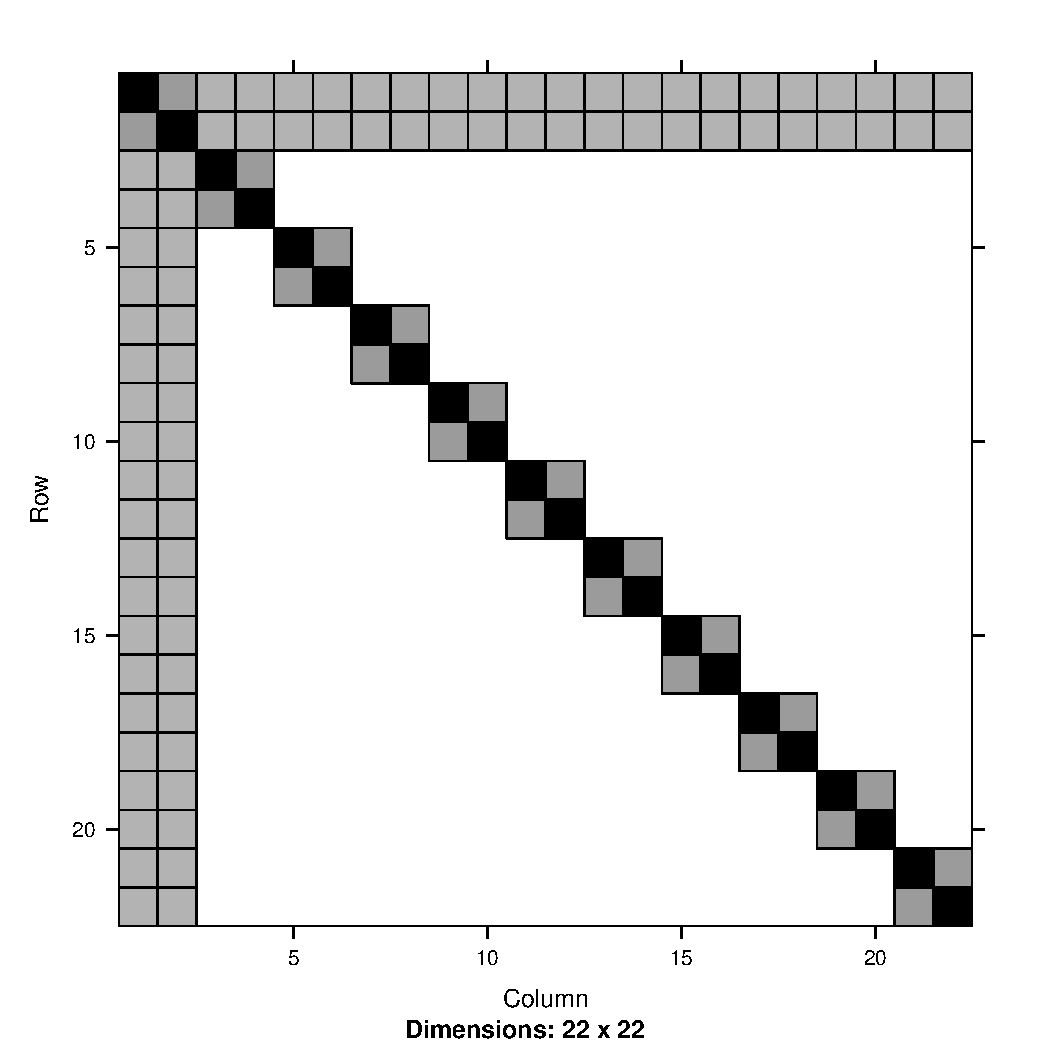
\includegraphics[scale=.15]{mX_mZ_mLambda.pdf}
		      		\caption{\tiny Covariance matrix -- Fixed effects before random effects}
		      	\end{subfigure}
		      	%
		      	\begin{subfigure}{0.4\textwidth}
		      		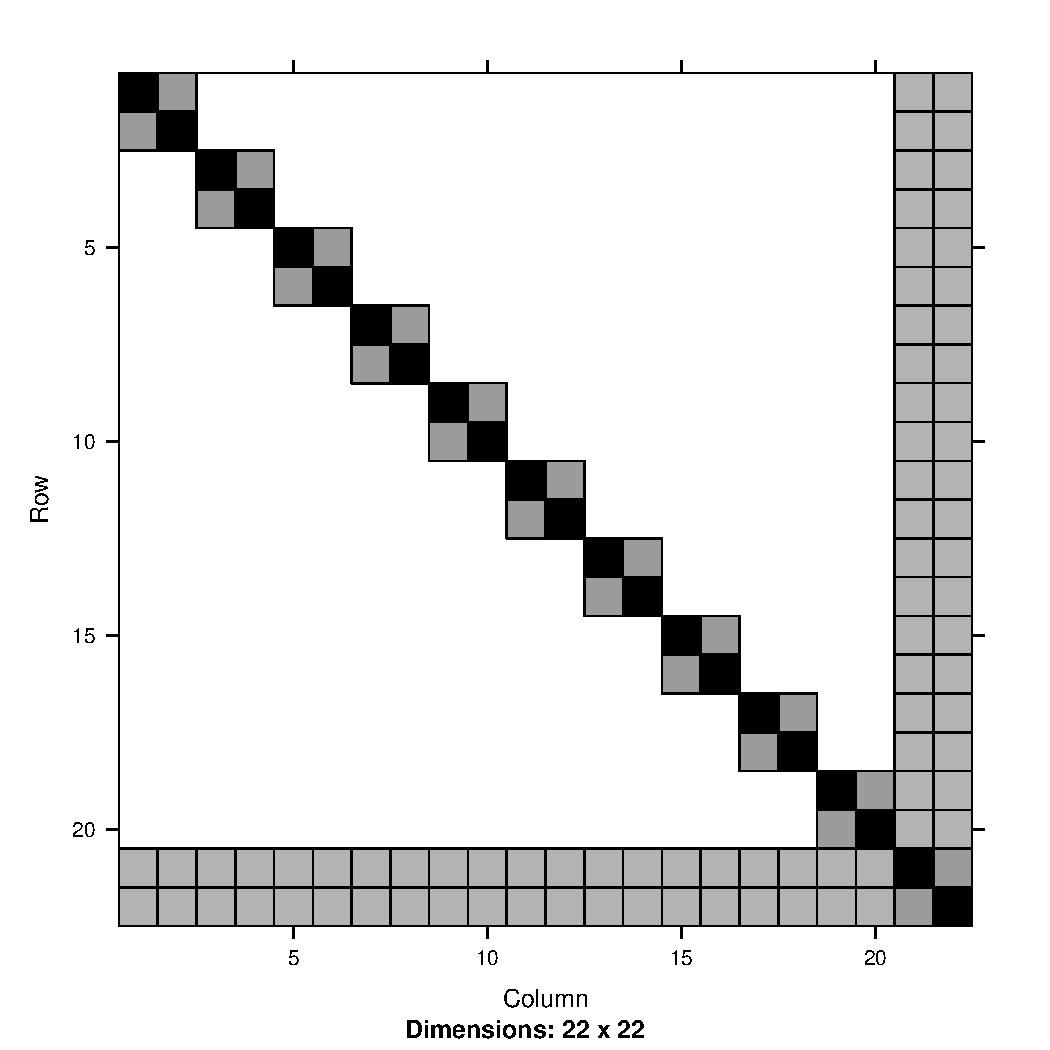
\includegraphics[scale=.15]{mZ_mX_mLambda.pdf}
		      		\caption{\tiny Covariance matrix -- Random effects before fixed effects}
		      	\end{subfigure}
		      			      	
		      	\begin{subfigure}{0.4\textwidth}
		      		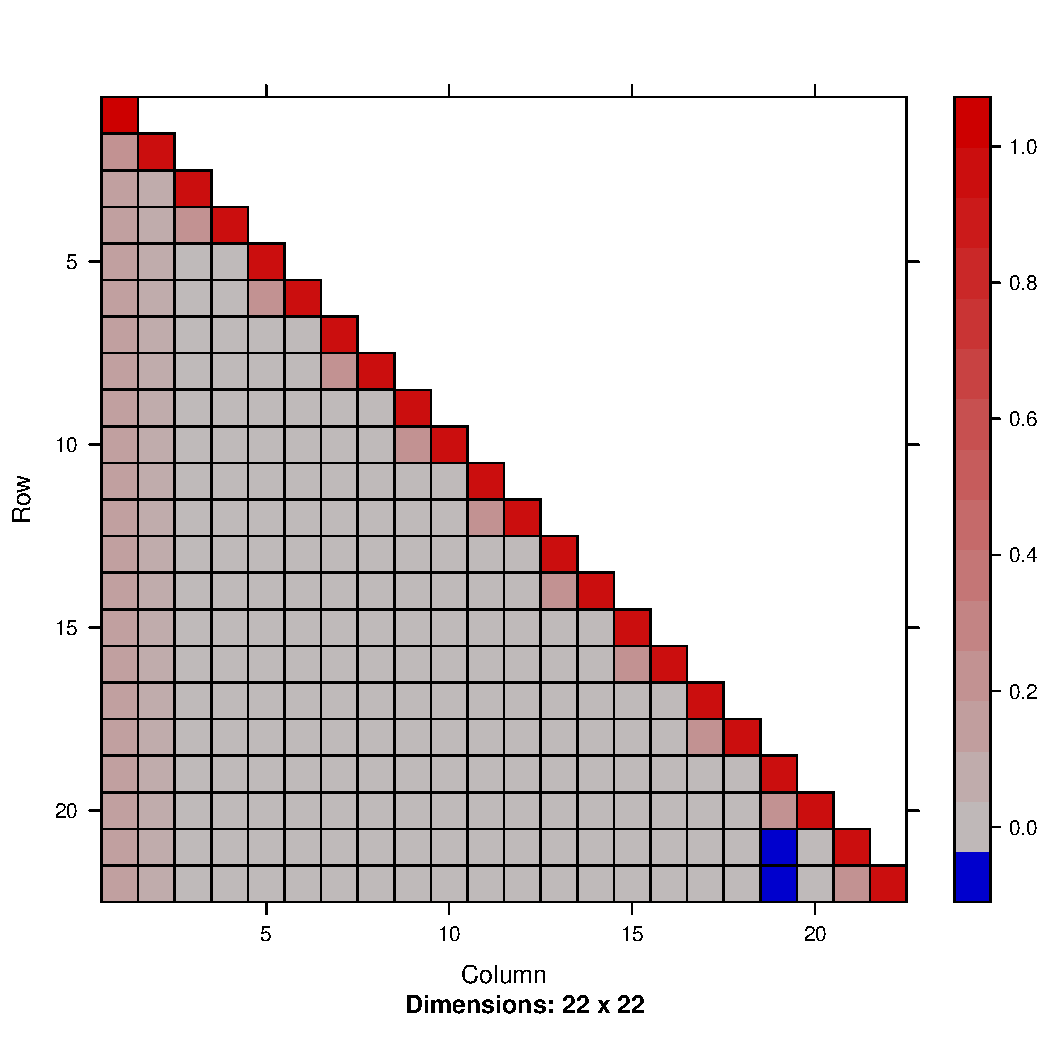
\includegraphics[scale=.15]{mX_mZ_cholesky.pdf}
		      		\caption{\tiny Cholesky factor -- Fixed effects before random effects}
		      	\end{subfigure}
		      	%
		      	\begin{subfigure}{0.4\textwidth}
		      		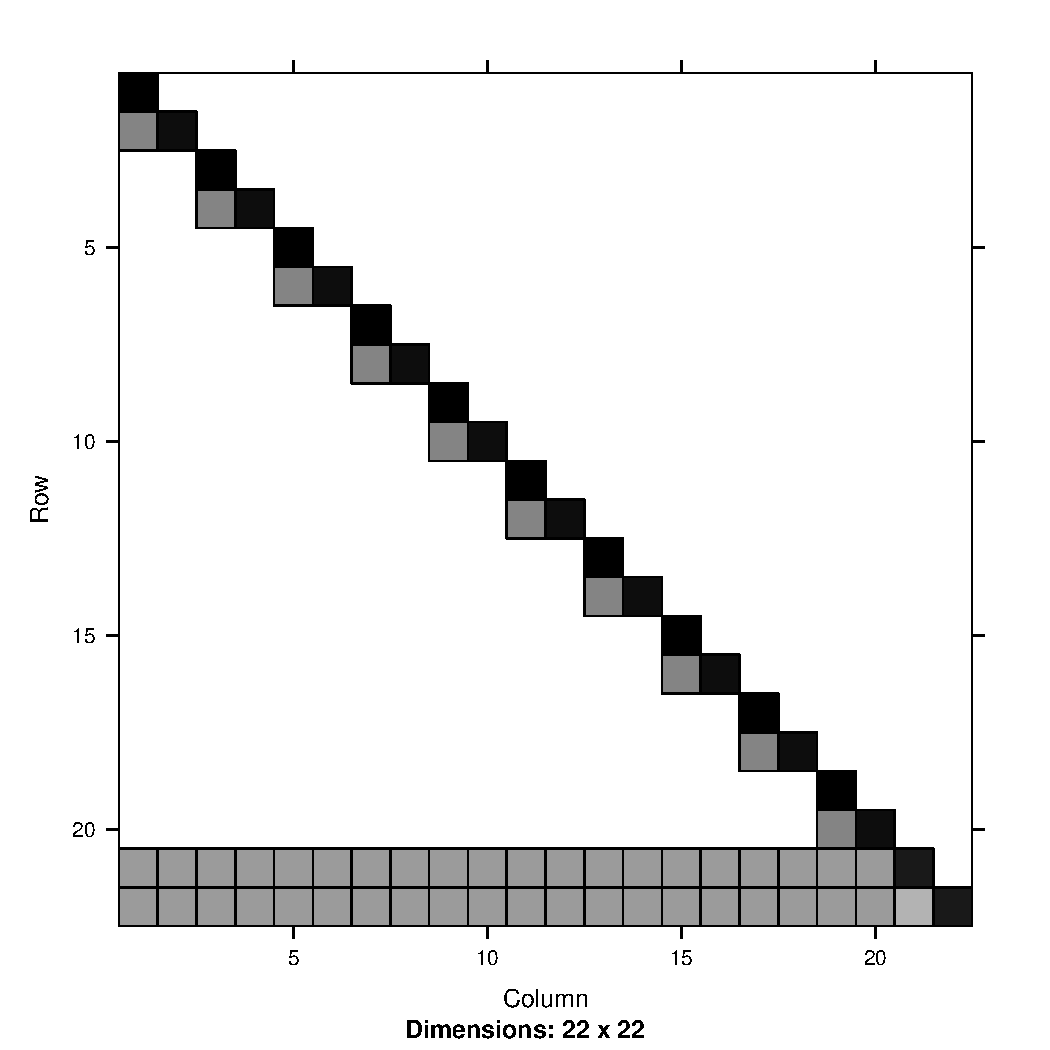
\includegraphics[scale=.15]{mZ_mX_cholesky.pdf}
		      		\caption{\tiny Cholesky factor -- Random effects before fixed effects}
		      	\end{subfigure}
		      \end{figure}
	\end{itemize}
\end{frame}

% \begin{frame}
% 	% Motivations behind the algorithms
% 	\frametitle{Motivations behind the algorithms}
% 	% ii) The Cholesky factor of a block matrix of the form
% 	% diag for random effects, block for cross effects
% 	% block for cross effects, diag for fixed effects
% 	% is mostly diagonal
% 	% Less parameters to optimise and store
% 	If we re-arrange the covariance matrix to have random effects before
% 	fixed effects, our posterior covariance matrix is of the form
% 	\begin{align*} \mLambda =
% 		\begin{pmatrix}
% 		\mLambda_{\vu_1 \vu_1}    & 0                      & \ldots & 0                          & \mLambda_{\vbeta_0 \vu_1}    & \mLambda_{\vbeta_1 \vu_1}    \\
% 		0                         & \mLambda_{\vu_2 \vu_2} & 0      & 0                          & \vdots                       & \vdots                       \\
% 		\vdots                    & 0                      & \ddots & 0                          & \vdots                       & \vdots                       \\
% 		0                         & 0                      & \ldots & \mLambda_{\vu_{m} \vu_{m}} & \mLambda_{\vbeta_0 \vu_{m}}  & \mLambda_{\vbeta_1 \vu_{m}}  \\
% 		\mLambda_{\vbeta_0 \vu_1} & \ldots                 & \ldots & \mLambda_{\vbeta_0 \vu_m}  & \mLambda_{\vbeta_0 \vbeta_0} & \mLambda_{\vbeta_0 \vbeta_1} \\
% 		\mLambda_{\vbeta_1 \vu_1} & \ldots                 & \ldots & \mLambda_{\vbeta_1 \vu_m}  & \mLambda_{\vbeta_1 \vbeta_0} & \mLambda_{\vbeta_1 \vbeta_1} 
% 		\end{pmatrix}
% 	\end{align*}
		
% 	As the $\sigma_{\vu^2}$ block is diagonal, the Cholesky factor is 
% 	sparse, with $\half m(m-1)$ zero elements. If $p$ is small
% 	and $m$ is large, as will typically be the case, then dimension of the parameter space of our optimisation
% 	problem will be much less.
% \end{frame}

% \begin{frame}
% 	\frametitle{L-BFGS-B}
% 	\begin{itemize}
% 		\item Approximate a smooth convex function locally with a quadratic form i.e. Taylor expand around the current point twice.
% 		      \[
% 		      	m_k(\vp) = f(\vx_k) + \nabla f(\vx_k)^\top \vp + \half \vp^\top \mB \vp
% 		      \]
% 		\item \begin{enumerate}
% 		\item Gradient and Hessian establish the direction of line search.
% 		\item Line search to find the best point in that direction.
% 		\end{enumerate}
% 		\item We used \texttt{optim} in base R, which tries lots of points alone the line, including some extreme 
% 		      ones.
% 		\item The parameterisation of the variational lower bound that we chose proved to be unstable in some 
% 		      regions. Much effort went into mitigating this.
% 	\end{itemize}
% \end{frame}

\begin{frame}
	\frametitle{Accuracy results using MCMC}
	\begin{itemize}
		\item	We measure the accuracy using
		      $$\text{Accuracy} = 1 - \half \int \left |p(\vtheta|\vy) - q(\vtheta) \right | d \vtheta.$$
		\item	$p(\vtheta|\vy)$ was estimated using the kernel density estimate of the posterior
		      distribution from MCMC.
		\item MCMC using 1 million iterations from Stan, about 8 CPU hours each.
		\item The need for approximate methods is obvious, this is simply not
		      practical for many types of applied work.
	\end{itemize}
\end{frame}

\begin{frame}
	\frametitle{Accuracy results}
	\begin{tabular}{|c|cccc|}
		\hline
		               & Laplacian & GVA                       & GVA                         & GVA NR \\
		               &           & $(\mLambda=\mR \mR^\top)$ & $[\mLambda=(\mR \mR)^{-1}]$ &        \\
		\hline
		$\vbeta_1$     & 0.84      & 0.94                      & 0.89                        & 0.94   \\
		$\vbeta_2$     & 0.85      & 0.99                      & 0.97                        & 0.99   \\
		$\vbeta_3$     & 0.85      & 0.97                      & 0.94                        & 0.97   \\
		$\vu_1$        & 0.86      & 0.95                      & 0.90                        & 0.95   \\
		$\vu_2$        & 0.88      & 0.95                      & 0.90                        & 0.95   \\
		$\vu_3$        & 0.83      & 0.94                      & 0.90                        & 0.94   \\
		$\vu_4$        & 0.58      & 0.93                      & 0.90                        & 0.93   \\
		$\vu_5$        & 0.75      & 0.88                      & 0.82                        & 0.88   \\
		$\vu_6$        & 0.62      & 0.83                      & 0.75                        & 0.83   \\
		$\vu_7$        & 0.87      & 0.94                      & 0.91                        & 0.94   \\
		$\vu_8$        & 0.83      & 0.97                      & 0.94                        & 0.97   \\
		$\vu_9$        & 0.65      & 0.84                      & 0.79                        & 0.84   \\
		$\vu_{10}$     & 0.84      & 0.96                      & 0.91                        & 0.96   \\
		$\vu_{11}$     & 0.84      & 0.95                      & 0.92                        & 0.95   \\
		$\vu_{12}$     & 0.79      & 0.96                      & 0.91                        & 0.96   \\
		$\sigma_\vu^2$ & 0.58      & 0.57                      & 0.62                        & 0.57   \\
		$\rho$         & 0.87      & 0.88                      & 0.87                        & 0.88   \\
		\hline
	\end{tabular}
\end{frame}

% Pretty pictures
\begin{frame}
	\frametitle{Plots of the MCMC-estimated and approximating densities}
	\begin{figure}
		\caption{Laplace's method}
		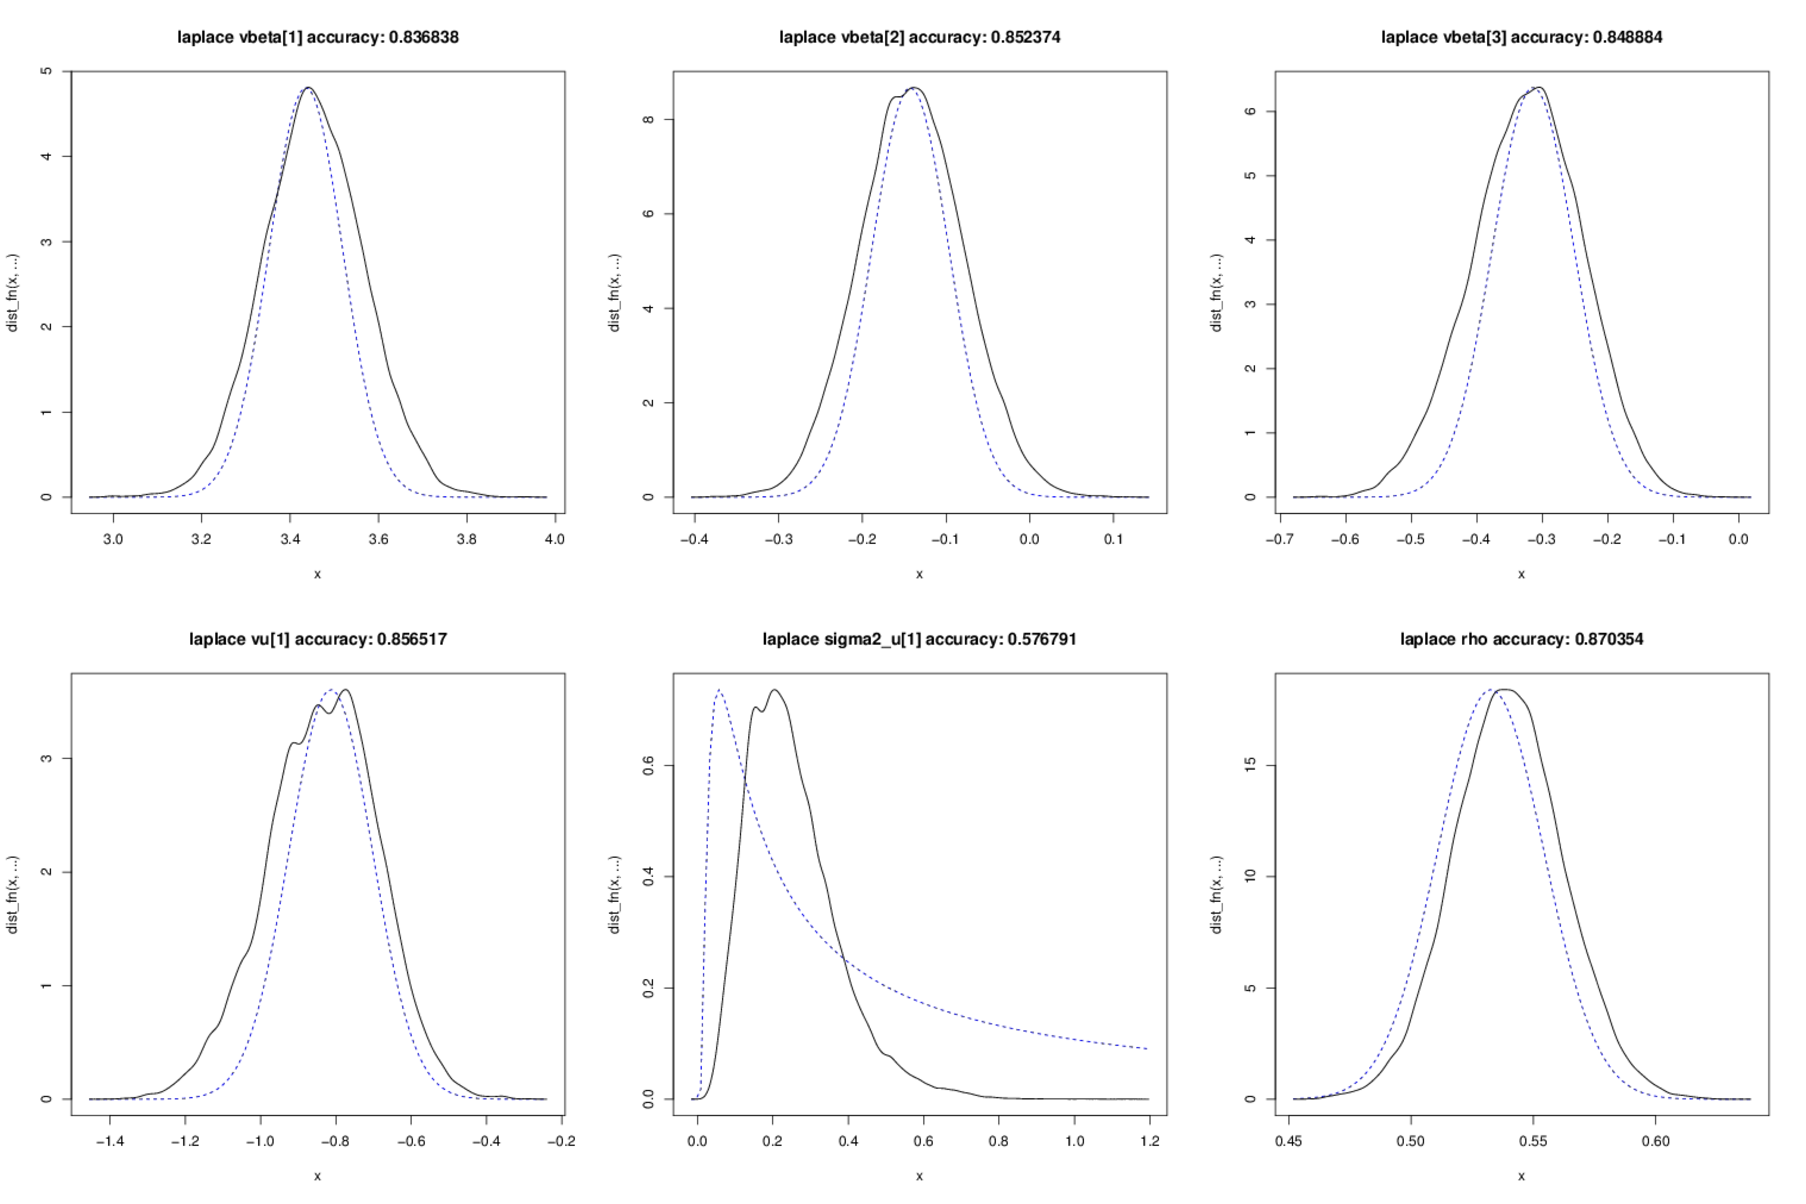
\includegraphics[scale=0.15]{code/results/output_montage_application_laplace.png}
	\end{figure}
\end{frame}

\begin{frame}
	\frametitle{Plots of the MCMC-estimated and approximating densities}
	\begin{figure}
		\caption{GVA ($\mLambda$ parameterisation)}
		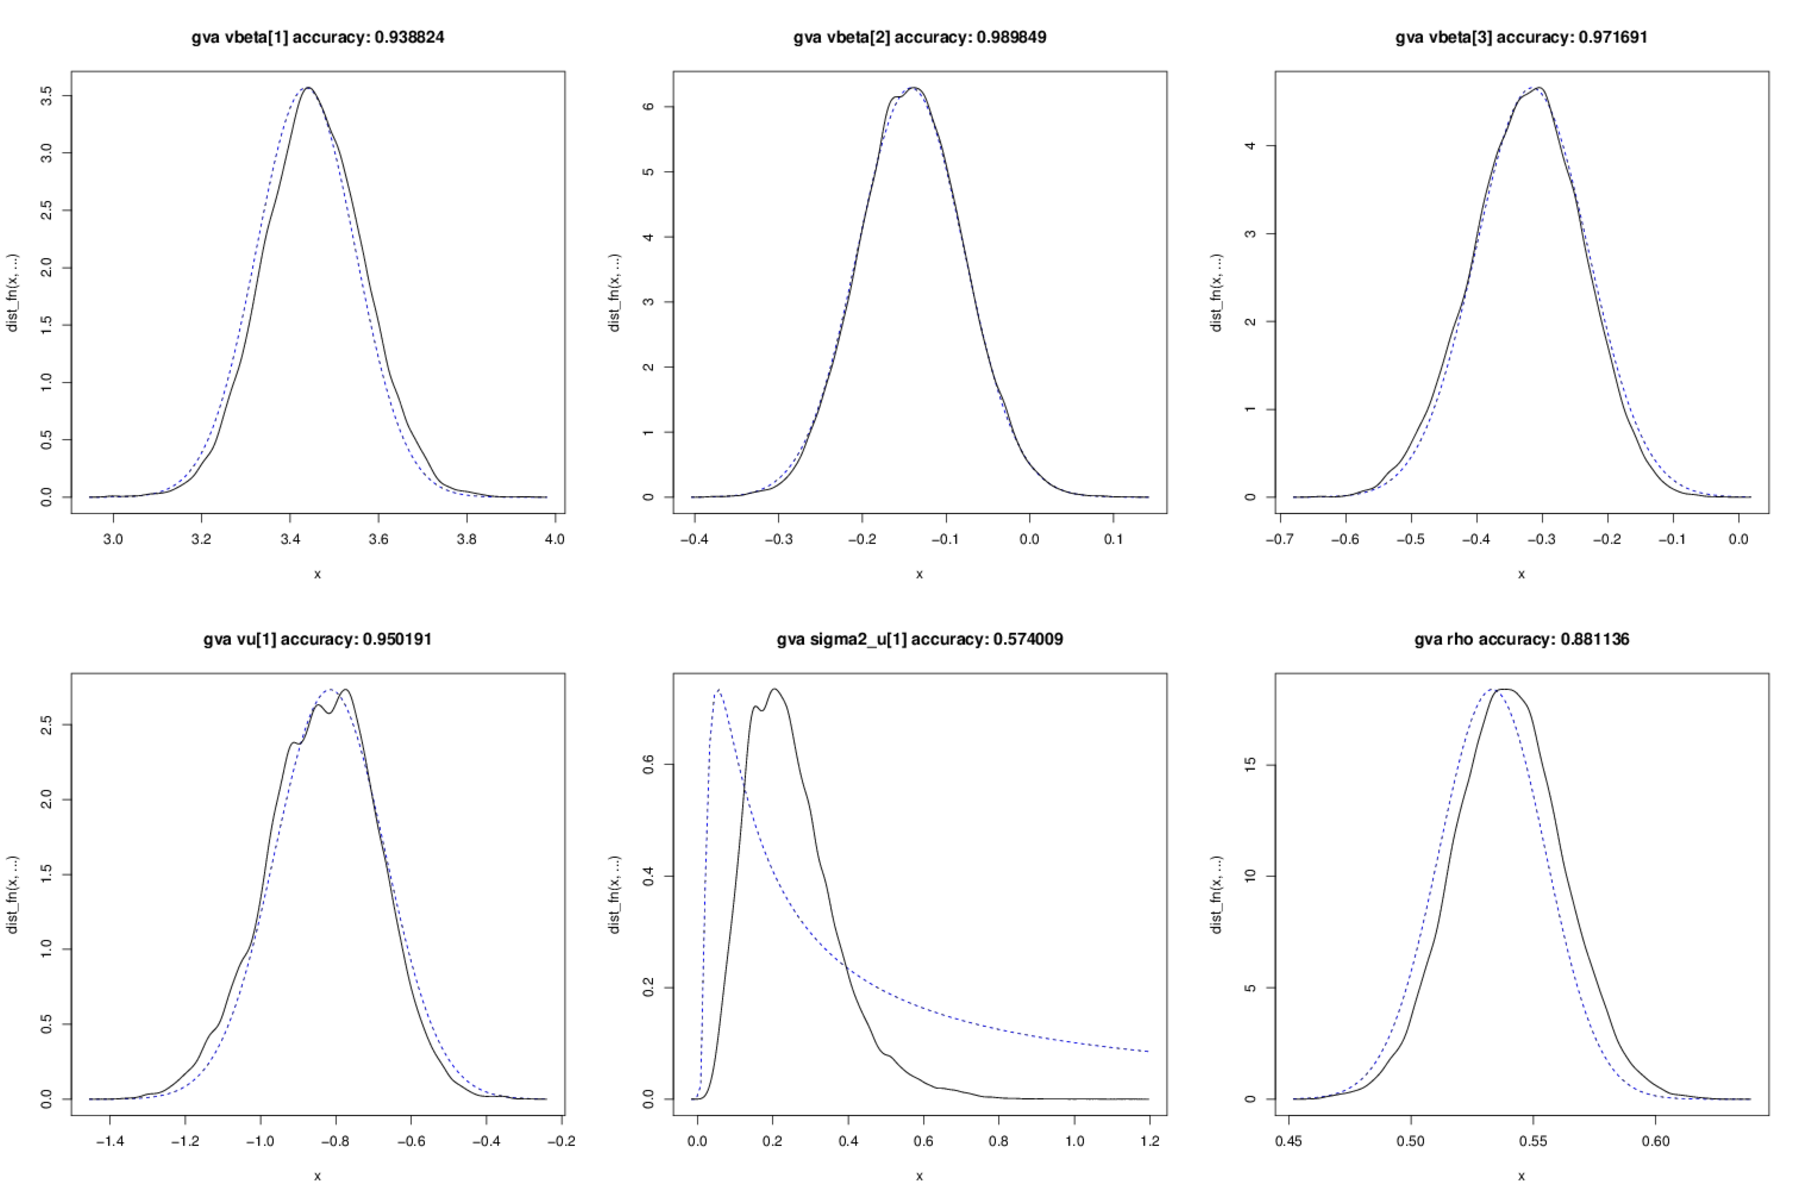
\includegraphics[scale=0.15]{code/results/output_montage_application_gva.png}
	\end{figure}
\end{frame}

% \begin{frame}
% 	\frametitle{Plots of the MCMC-estimated and approximating densities}
% 	\begin{figure}
% 		\caption{GVA ($\mLambda^{-1}$ parameterisation)}
% 		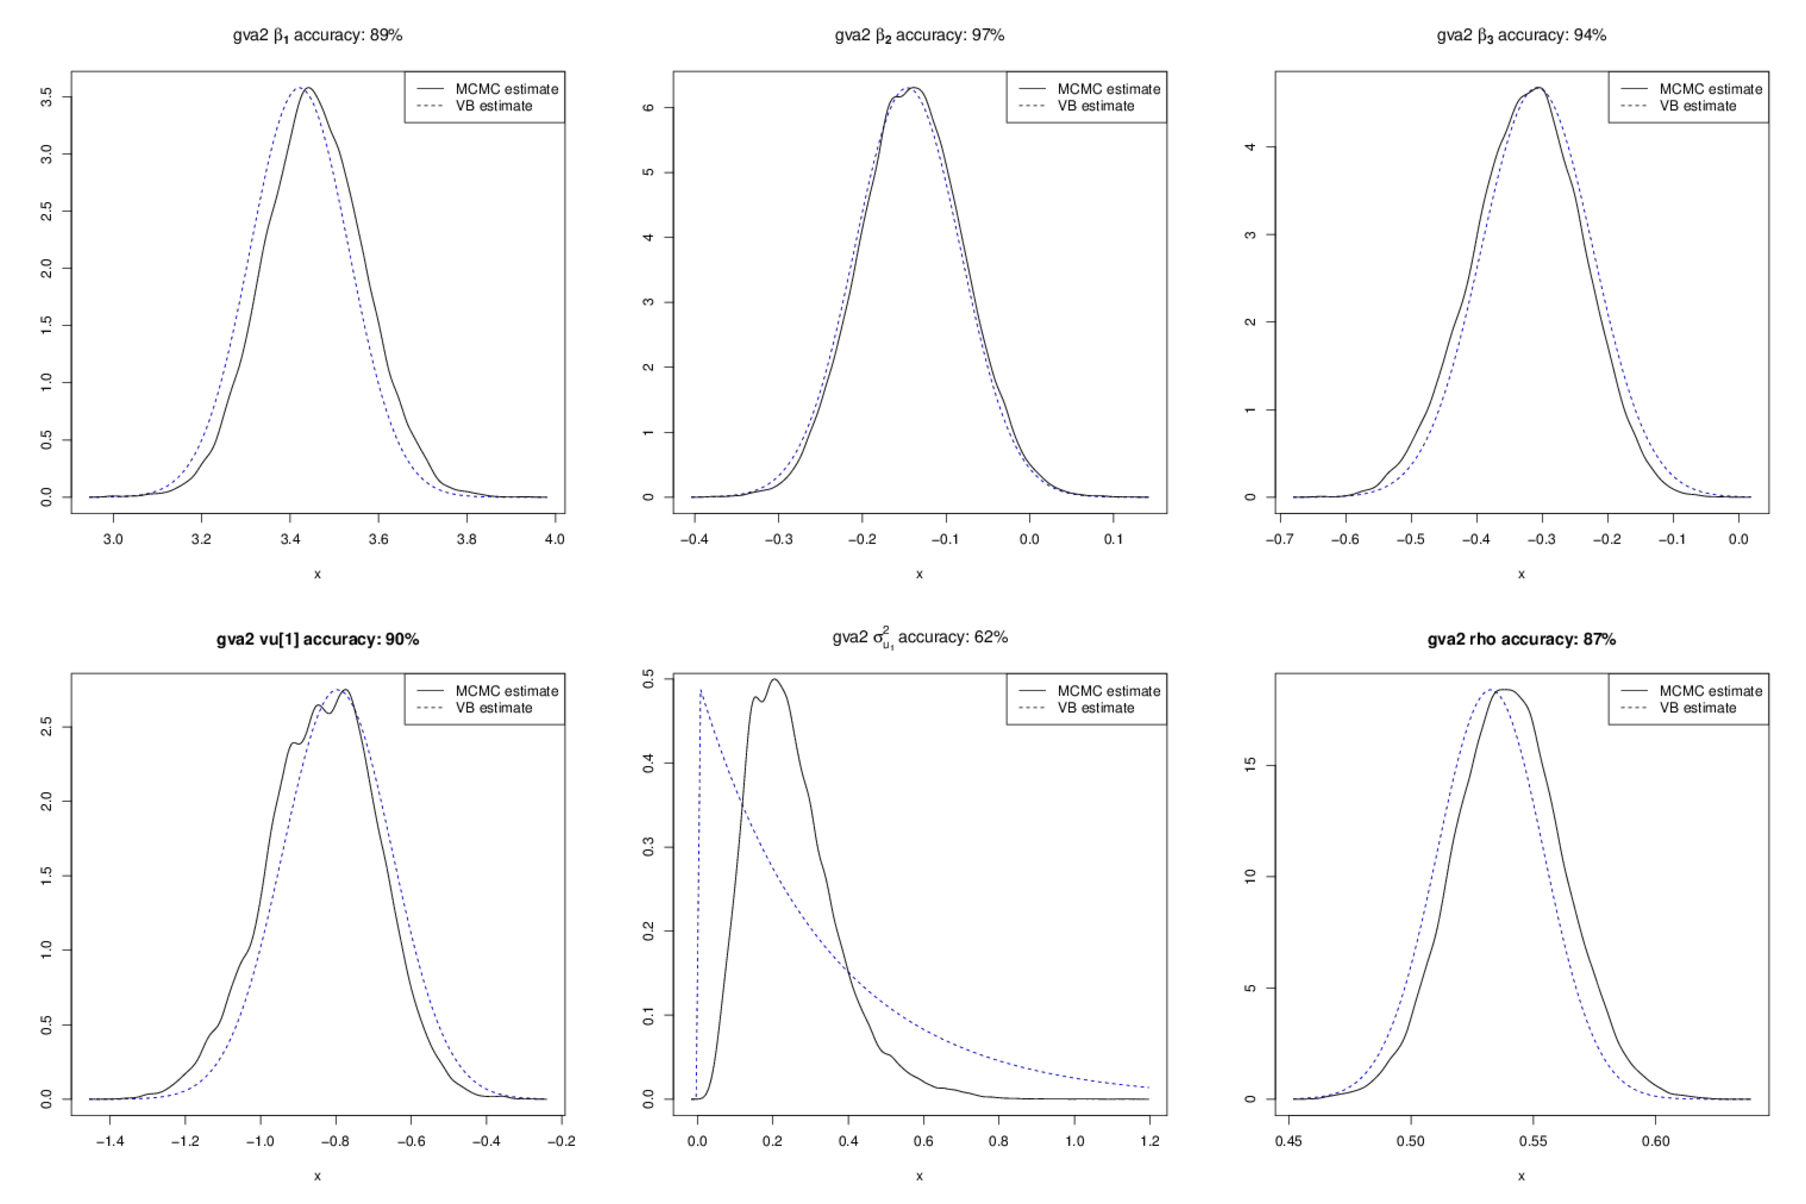
\includegraphics[scale=0.15]{code/results/output_montage_application_gva2.png}
% 	\end{figure}
% \end{frame}

% \begin{frame}
% 	\frametitle{Plots of the MCMC-estimated and approximating densities}
% 	\begin{figure}
% 		\caption{GVA Newton-Raphson}
% 		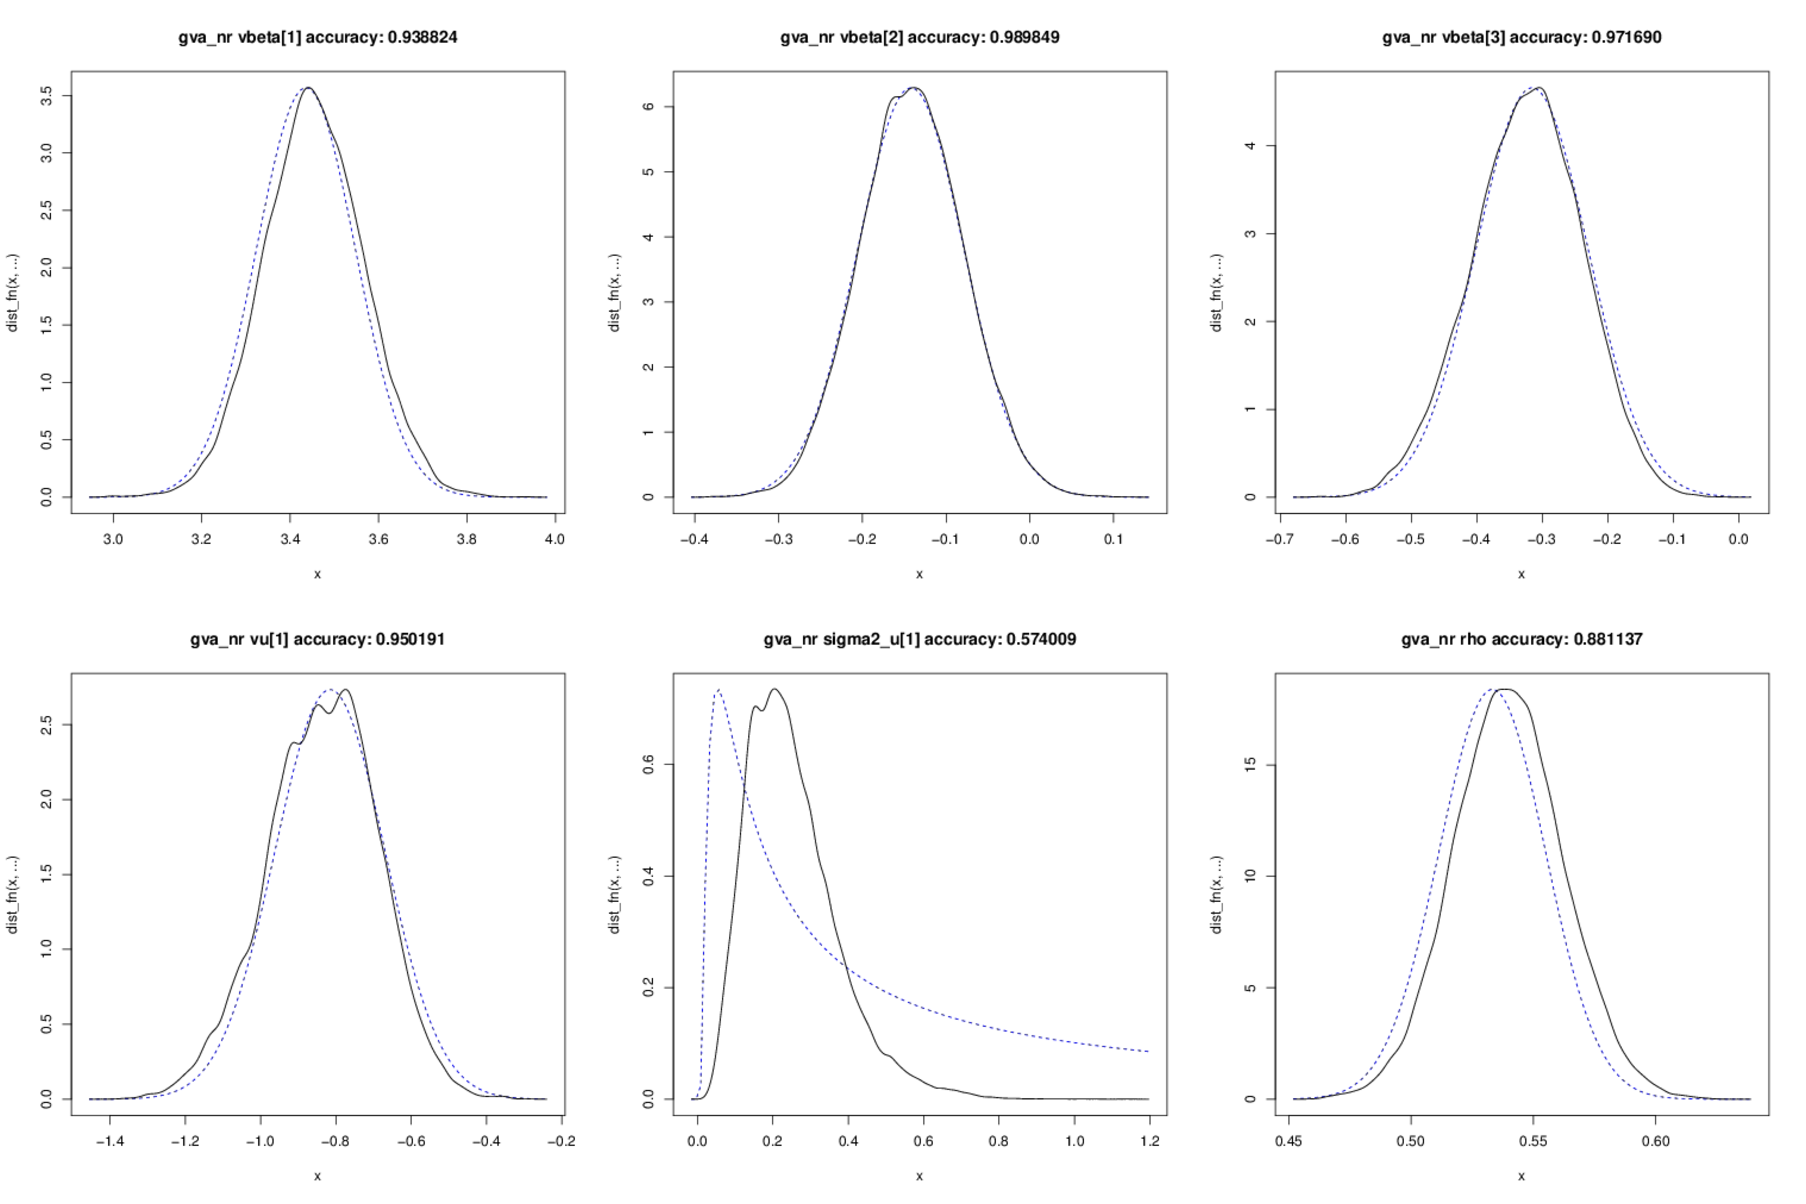
\includegraphics[scale=0.15]{code/results/output_montage_application_gva_nr.png}
% 	\end{figure}
% \end{frame}

\begin{frame}{R package}
	\begin{itemize}
		\item I'm intending to release the \texttt{zipvb} on GitHub when it's ready.
		\item Interface modelled on \texttt{lme4}.
		\item Currently, random intercepts and random slopes are supported.
		\item Splines are also supported.
	\end{itemize}	
\end{frame}

\begin{frame}
	\frametitle{References}
	\begin{itemize}
		\item Explaining Variational Approximations, J.T. Ormerod, M.P. Wand, American Statistician, 2010
		\item Gaussian Variational Approximations, J.T. Ormerod, M.P. Wand, , Journal of Computational Statistics, 2012
		\item General Design Mixed Models, M.P. Wand and others, Statistical Science, 2006, 
		\item Numerical Optimisation, Nocedal and Wright, Textbook, 1999
	\end{itemize}
\end{frame}

\end{document}
